% =============================================================================
% MaudeIR Language Reference
% A Domain-Specific Language for Protocol Modeling and Formal Verification
% =============================================================================
\documentclass[11pt,letterpaper]{article}

% ── Packages ─────────────────────────────────────────────────────────────────
\usepackage[utf8]{inputenc}
\usepackage[T1]{fontenc}
\usepackage{lmodern}
\usepackage[margin=1in]{geometry}
\usepackage{hyperref}
\usepackage{xcolor}
\usepackage{listings}
\usepackage{booktabs}
\usepackage{longtable}
\usepackage{enumitem}
\usepackage{fancyhdr}
\usepackage{titlesec}
\usepackage{tcolorbox}
\usepackage{amsmath,amssymb}
\usepackage{tikz}
\usetikzlibrary{automata,positioning,arrows.meta}

% ── Colours ──────────────────────────────────────────────────────────────────
\definecolor{keyword}{RGB}{0,112,192}
\definecolor{string}{RGB}{163,21,21}
\definecolor{comment}{RGB}{106,153,85}
\definecolor{bg}{RGB}{248,248,248}
\definecolor{frame}{RGB}{200,200,200}
\definecolor{accentblue}{RGB}{0,99,177}

% ── Listings style ───────────────────────────────────────────────────────────
\lstdefinelanguage{MaudeIR}{
  morekeywords={import,config,type,struct,event,function,nondet,machine,
                state,initial,transition,on,test,assert,if,for,in,
                return,and,or,log,del,len,choice,True,False},
  sensitive=true,
  morecomment=[l]{//},
  morecomment=[s]{/*}{*/},
  morestring=[b]",
  literate={->}{$\rightarrow$}2
           {==}{==}2
           {!=}{!=}2
           {<=}{$\leq$}2
           {>=}{$\geq$}2,
}

\lstset{
  language=MaudeIR,
  backgroundcolor=\color{bg},
  frame=single,
  rulecolor=\color{frame},
  basicstyle=\ttfamily\small,
  keywordstyle=\bfseries\color{keyword},
  stringstyle=\color{string},
  commentstyle=\itshape\color{comment},
  breaklines=true,
  showstringspaces=false,
  tabsize=4,
  numbers=left,
  numberstyle=\tiny\color{gray},
  numbersep=8pt,
  xleftmargin=1.2em,
  framexleftmargin=0.8em,
  captionpos=b,
}

% ── Tip / Note boxes ────────────────────────────────────────────────────────
\newtcolorbox{notebox}{
  colback=blue!5,colframe=accentblue,
  fonttitle=\bfseries,title=Note,
  left=6pt,right=6pt,top=4pt,bottom=4pt
}

\newtcolorbox{tipbox}{
  colback=green!5,colframe=green!50!black,
  fonttitle=\bfseries,title=Tip,
  left=6pt,right=6pt,top=4pt,bottom=4pt
}

\newtcolorbox{warningbox}{
  colback=red!5,colframe=red!60!black,
  fonttitle=\bfseries,title=Warning,
  left=6pt,right=6pt,top=4pt,bottom=4pt
}

\newtcolorbox{syntaxbox}[1][]{
  colback=bg,colframe=frame,
  fonttitle=\bfseries\ttfamily,title=#1,
  left=6pt,right=6pt,top=4pt,bottom=4pt
}

% ── Header / Footer ─────────────────────────────────────────────────────────
\pagestyle{fancy}
\fancyhf{}
\fancyhead[L]{\small\textsc{MaudeIR Language Reference}}
\fancyhead[R]{\small\thepage}
\renewcommand{\headrulewidth}{0.4pt}

% ── Section formatting ──────────────────────────────────────────────────────
\titleformat{\section}
  {\Large\bfseries\color{accentblue}}{\thesection}{1em}{}
\titleformat{\subsection}
  {\large\bfseries\color{accentblue!80!black}}{\thesubsection}{1em}{}
\titleformat{\subsubsection}
  {\normalsize\bfseries}{\thesubsubsection}{1em}{}

% ── Hyperref setup ──────────────────────────────────────────────────────────
\hypersetup{
  colorlinks=true,
  linkcolor=accentblue,
  urlcolor=accentblue,
  citecolor=accentblue,
  pdftitle={MaudeIR Language Reference},
  pdfauthor={Proto-IR Project},
}

% ═════════════════════════════════════════════════════════════════════════════
\begin{document}

% ── Title page ──────────────────────────────────────────────────────────────
\begin{titlepage}
\centering
\vspace*{3cm}
{\Huge\bfseries MaudeIR\\[0.3em]Language Reference\par}
\vspace{1cm}
{\Large A Domain-Specific Language for\\Protocol Modeling \& Formal Verification\par}
\vspace{2cm}
{\large Version 1.0\par}
\vspace{0.5cm}
{\large\today\par}
\vfill
{\small Proto-IR Project}
\end{titlepage}

% ── Table of contents ───────────────────────────────────────────────────────
\tableofcontents
\newpage

% ═════════════════════════════════════════════════════════════════════════════
\section{Introduction}
\label{sec:introduction}

MaudeIR is a domain-specific language (DSL) for specifying communicating
state-machine protocols and subjecting them to repeatable, automated
verification.  A single \texttt{.model} source file captures data types,
events, machines, and executable tests.  The toolchain then provides three
complementary workflows:

\begin{enumerate}
  \item \textbf{Simulation}\,---\,a built-in Python interpreter executes
        tests against the model, dispatching events across machine instances
        and checking assertions.
  \item \textbf{Transpilation}\,---\,a compiler translates the model into
        Maude rewriting-logic modules, enabling unbounded state-space
        exploration and model checking via the Maude system.
  \item \textbf{Visualization}\,---\,each machine's state graph is
        rendered as a Graphviz diagram for documentation and review.
\end{enumerate}

\subsection{Design Goals}
\begin{itemize}[leftmargin=1.5em]
  \item \textbf{Clarity.}  Protocol specifications should read like
        structured pseudocode, not rewriting-logic equations.
  \item \textbf{Soundness.}  Every syntactically valid model has a
        well-defined operational semantics in both the simulator and the
        generated Maude theory.
  \item \textbf{Composability.}  Models are split across files via
        \lstinline{import} and composed at parse time through automatic
        dependency resolution.
  \item \textbf{Testability.}  An integrated test framework lets authors
        assert reachability properties before committing to a full formal
        verification pass.
\end{itemize}

\subsection{Intended Audience}

This reference targets engineers and researchers with background in
protocol design or formal methods.  Familiarity with state-machine
formalisms (e.g., Mealy/Moore machines, CSP, rewriting logic) is
helpful but not required.


% ═════════════════════════════════════════════════════════════════════════════
\section{Getting Started}
\label{sec:getting-started}

\subsection{Prerequisites}
\begin{itemize}[leftmargin=1.5em]
  \item Python~3.8 or later.
  \item \texttt{pip} packages: \texttt{lark} (parser generator), optionally
        \texttt{pyyaml} (for YAML configurations) and \texttt{graphviz}
        (Python bindings).
  \item \emph{Optional:} the Graphviz \texttt{dot} binary, required only for
        the \texttt{-g} visualization flag.
  \item \emph{Optional:} the
        \href{http://maude.cs.illinois.edu}{Maude} system, required only for
        executing the transpiled output.
\end{itemize}

\subsection{Installation}
\begin{lstlisting}[language=bash,numbers=none]
# Create and activate a virtual environment
python3 -m venv venv
source venv/bin/activate      # macOS / Linux

# Install dependencies
pip install -r requirements.txt
\end{lstlisting}

\subsection{Quick Start}

Given a project with the following layout:

\begin{lstlisting}[language=bash,numbers=none]
my_protocol/
  common.model            # shared struct definitions
  server.model            # server machine
  client.model            # client machine
  main.model              # imports + tests
  config.yaml             # runtime parameters
\end{lstlisting}

Run the toolchain:

\begin{lstlisting}[language=bash,numbers=none]
python3 transpile.py my_protocol/main.model \
    -c my_protocol/config.yaml \
    -o output/
\end{lstlisting}

This will:
\begin{enumerate}
  \item Parse all \texttt{.model} files reachable from
        \texttt{main.model}.
  \item Run semantic validation.
  \item Execute the built-in simulation tests and report pass/fail
        results.
  \item Write transpiled Maude modules to the \texttt{output/}
        directory.
\end{enumerate}


% ═════════════════════════════════════════════════════════════════════════════
\section{Lexical Structure}
\label{sec:lexical}

\subsection{Character Set and Encoding}

Source files must be encoded in UTF-8.

\subsection{Identifiers}

Identifiers follow the C naming convention: a letter or underscore,
followed by zero or more letters, digits, or underscores.  Identifiers are
case-sensitive.

\begin{syntaxbox}[CNAME]
\texttt{[a-zA-Z\_][a-zA-Z0-9\_]*}
\end{syntaxbox}

\subsection{Keywords}

The following tokens are reserved and may not be used as identifiers:

\begin{center}
\begin{tabular}{llllll}
\toprule
\texttt{import} & \texttt{config}   & \texttt{type}     & \texttt{struct}  & \texttt{event}    & \texttt{function} \\
\texttt{nondet} & \texttt{machine}  & \texttt{state}    & \texttt{initial} & \texttt{transition} & \texttt{on}  \\
\texttt{test}   & \texttt{assert}   & \texttt{if}       & \texttt{for}     & \texttt{in}       & \texttt{return} \\
\texttt{and}    & \texttt{or}       & \texttt{True}     & \texttt{False}   &                   & \\
\bottomrule
\end{tabular}
\end{center}

\subsection{Literals}

\subsubsection{Numeric Literals}
Integer and floating-point literals are supported using the standard
signed-number format: \texttt{42}, \texttt{-7}, \texttt{3.14}.

\subsubsection{String Literals}
Strings are delimited by double quotes.  Standard C escape sequences are
supported (e.g., \texttt{\textbackslash n}, \texttt{\textbackslash t}).
String interpolation is supported inside \lstinline{log()} calls using
curly braces: \lstinline{"Value is {x}"}.

\subsubsection{Boolean Literals}
The tokens \lstinline{True} and \lstinline{False} denote boolean values.

\subsection{Comments}

MaudeIR supports two comment styles:

\begin{lstlisting}[numbers=none]
// Single-line comment

/* Multi-line
   comment */
\end{lstlisting}

\subsection{Whitespace}

Whitespace (spaces, tabs, newlines) is ignored between tokens and serves
only to separate adjacent identifiers or keywords.


% ═════════════════════════════════════════════════════════════════════════════
\section{Type System}
\label{sec:types}

\subsection{Primitive Types}

\begin{longtable}{@{}llp{7.8cm}@{}}
\toprule
\textbf{Type}    & \textbf{Maude Sort} & \textbf{Description} \\
\midrule
\texttt{Int}     & \texttt{Int}        & Arbitrary-precision integer. \\
\texttt{String}  & \texttt{String}     & UTF-8 text. \\
\texttt{Bool}    & \texttt{Bool}       & Boolean (\texttt{True}/\texttt{False}). \\
\texttt{Object}  & \texttt{Oid}        & Object identifier (Maude). \\
\texttt{None}    & ---                 & Unit type for side-effecting functions. \\
\bottomrule
\end{longtable}

\subsection{Generic Types}

Type expressions support one level of generic parameterization using
bracket notation:

\begin{syntaxbox}[Type Expression Syntax]
\texttt{type\_expr ::= CNAME ( "[" type\_expr ("," type\_expr)* "]" )?}
\end{syntaxbox}

\textbf{Examples:}
\begin{lstlisting}[numbers=none]
List[IRCClient]
Map[String, Int]
\end{lstlisting}

In the current implementation, the simulator interprets \texttt{List[T]}
as a Python list and \texttt{Map[K,V]} as a Python dictionary.  The
transpiler maps lists and maps to Maude algebraic data types with
\texttt{putMap}/\texttt{getMap} operations.

\subsection{Type Aliases}

The \lstinline{type} declaration introduces a named alias for an existing
type expression.

\begin{syntaxbox}[type]
\texttt{type} \textit{Name} \texttt{=} \textit{TypeExpr}
\end{syntaxbox}

\textbf{Example:}
\begin{lstlisting}[numbers=none]
type NodeID = String
\end{lstlisting}


% ═════════════════════════════════════════════════════════════════════════════
\section{Top-Level Declarations}
\label{sec:declarations}

A MaudeIR source file consists of a sequence of top-level declarations.
Declarations may appear in any order, subject to the constraint that
an identifier must be defined before it is referenced across file
boundaries (resolved automatically by the import system).

\begin{syntaxbox}[Top-Level Grammar]
\texttt{start ::= statement*} \\
\texttt{statement ::= import\_stmt | config\_stmt | type\_decl |} \\
\hspace*{4em}\texttt{struct\_decl | event\_decl | func\_decl |} \\
\hspace*{4em}\texttt{machine\_decl | test\_decl}
\end{syntaxbox}

\subsection{Import Declarations}
\label{sec:imports}

\begin{syntaxbox}[import]
\texttt{import} \textit{"relative/path.model"}
\end{syntaxbox}

Imports are resolved at parse time relative to the directory of the
importing file.  The parser performs recursive, cycle-safe resolution:
each file is parsed at most once, and its declarations are merged into
the combined program AST.

\textbf{Example:}
\begin{lstlisting}[numbers=none]
import "common.model"
import "irc_server.model"
\end{lstlisting}

\subsection{Configuration Parameters}
\label{sec:config}

\begin{syntaxbox}[config]
\texttt{config} \textit{MachineName}\texttt{.}\textit{fieldName} \texttt{:} \textit{TypeExpr}
\end{syntaxbox}

Configuration parameters declare externally provided values that are
bound at compile time via a YAML or JSON configuration file passed on
the command line.  They are scoped by machine name and are available
within transitions of the named machine as local variables.

\textbf{Example:}
\begin{lstlisting}[numbers=none]
config NetworkChannel.minDelay: Int
config NetworkChannel.maxDelay: Int
\end{lstlisting}

Corresponding \texttt{config.yaml}:
\begin{lstlisting}[language=bash,numbers=none]
NetworkChannel.minDelay: 100
NetworkChannel.maxDelay: 500
\end{lstlisting}


% ═════════════════════════════════════════════════════════════════════════════
\section{Struct Declarations}
\label{sec:structs}

\begin{syntaxbox}[struct]
\texttt{struct} \textit{Name} \texttt{\{} \\
\hspace*{2em}\textit{fieldName} \texttt{:} \textit{TypeExpr} \\
\hspace*{2em}\textit{...} \\
\texttt{\}}
\end{syntaxbox}

Structs define product types.  Each field has a name and a type
expression.  Struct values are constructed positionally.

\textbf{Example:}
\begin{lstlisting}
struct Message {
    command: String
    payload: String
}
\end{lstlisting}

\subsubsection{Struct Construction}

Struct instances are created by calling the struct name with positional
arguments matching the field order:

\begin{lstlisting}[numbers=none]
msg = Message("CONNECT", "hello")
\end{lstlisting}

\subsubsection{Field Access}

Fields are accessed using dot notation:

\begin{lstlisting}[numbers=none]
msg.command    // evaluates to "CONNECT"
msg.payload    // evaluates to "hello"
\end{lstlisting}

In the generated Maude output, field access is implemented via
automatically generated projection functions:
\texttt{command(msg)} $\Rightarrow$ \texttt{"CONNECT"}.

\subsubsection{Struct Matching in Transitions}

Struct patterns can be used in event arguments within transitions to
destructure incoming values:

\begin{lstlisting}[numbers=none]
transition S on receive(msg: Message { command: "ACK" }) -> S2 {
    // Only matches if msg.command == "ACK"
}
\end{lstlisting}


% ═════════════════════════════════════════════════════════════════════════════
\section{Event Declarations}
\label{sec:events}

\begin{syntaxbox}[event]
\texttt{event} \textit{Name}\texttt{(} \textit{param} \texttt{:} \textit{Type}\texttt{,} \textit{...} \texttt{)}
\end{syntaxbox}

Events declare the messages that a machine can receive.  Each event has a
name and a typed parameter list.  Events can be declared at the top level
(global scope) or inside a \lstinline{machine} body.

\textbf{Example:}
\begin{lstlisting}[numbers=none]
event receive(client: IRCClient, msg: Message)
\end{lstlisting}

Events declared inside a machine define the interface that other machines
use to communicate with it.  The simulator uses the parameter count to
determine whether an implicit caller reference should be injected.


% ═════════════════════════════════════════════════════════════════════════════
\section{Function Declarations}
\label{sec:functions}

\begin{syntaxbox}[function]
\texttt{[nondet] function} \textit{Name}\texttt{(} \textit{params} \texttt{)} \texttt{->} \textit{ReturnType}
  \texttt{[\{} \textit{body} \texttt{\}]}
\end{syntaxbox}

Functions define reusable computations.  They may appear at the top level
or inside a machine body.

\subsection{Function Parameters and Return Type}

Parameters are comma-separated \texttt{name: Type} pairs.  The return
type follows the \lstinline{->} arrow.  Use \texttt{None} for
side-effecting functions that return no value.

\subsection{Function Body}

A function body is a sequence of action statements enclosed in braces.
If the body is omitted, the function acts as a \emph{declaration-only}
signature; the transpiler emits a mock equation that returns a
type-appropriate default value.

\textbf{Example~--- concrete function:}
\begin{lstlisting}
function broadcast(client: IRCClient, msg: Message) -> None {
    for peer in connections {
        if (peer != client) {
            peer.receive(msg)
        }
    }
}
\end{lstlisting}

\textbf{Example~--- declaration-only:}
\begin{lstlisting}[numbers=none]
function createTimer(delay: Int) -> String
\end{lstlisting}

\subsection{Nondeterministic Functions}
\label{sec:nondet}

Prefixing a function declaration with the \lstinline{nondet} keyword marks
it as nondeterministic.  This signals two things:

\begin{enumerate}
  \item \textbf{Simulator:}  The function returns a deterministic mock
        value (e.g., \texttt{42} for \texttt{Int}).  Any test that
        exercises a nondeterministic function will print a warning.
  \item \textbf{Transpiler:}  The Maude output converts each call site
        into a fresh \emph{choice variable} with rewriting-logic
        constraints, enabling the Maude search command to explore all
        possible return values within the specified range.
\end{enumerate}

\textbf{Example:}
\begin{lstlisting}[numbers=none]
nondet function randInt(min: Int, max: Int) -> Int
nondet function randCommand() -> String
\end{lstlisting}

\subsection{Machine-Scoped Functions}

Functions declared inside a machine body have access to the machine's
instance variables via an implicit \texttt{self} reference.  Calls to
machine-scoped functions are dispatched on the target machine instance:

\begin{lstlisting}[numbers=none]
machine IRCClient {
    function connect(server: IRCServer) -> None {
        server.receive(Message("CONNECT", nick))
    }
}

// In a test:
client1.connect(server)
\end{lstlisting}


% ═════════════════════════════════════════════════════════════════════════════
\section{Machine Declarations}
\label{sec:machines}

Machines are the central modeling primitive in MaudeIR.  Each machine
declaration defines a communicating finite-state automaton with typed
instance variables, named states, and guarded transitions.

\begin{syntaxbox}[machine]
\texttt{machine} \textit{Name} \texttt{[(} \textit{params} \texttt{)]}
  \texttt{\{} \textit{members} \texttt{\}}
\end{syntaxbox}

\subsection{Machine Parameters}

A machine may accept construction-time parameters.  These are bound when
the machine is instantiated in a test.

\begin{lstlisting}[numbers=none]
machine IRCClient (client_id: String) {
    nick: String = client_id
    ...
}
\end{lstlisting}

\subsection{Instance Variables}

\begin{syntaxbox}[Variable Declaration]
\texttt{name : TypeExpr [ = expr ]}
\end{syntaxbox}

Variables declare the mutable state of a machine instance.  Each variable
has a type and an optional initializer expression.  Variables of type
\texttt{List[T]} are initialized to the empty list by default if no
initializer is provided.

\textbf{Example:}
\begin{lstlisting}[numbers=none]
connections: List[IRCClient]
nick: String = "server"
\end{lstlisting}

\subsection{State Declarations}

\begin{syntaxbox}[state / initial]
\texttt{state} \textit{Name} \\
\texttt{initial} \textit{Name}
\end{syntaxbox}

States are named constants.  The \lstinline{initial} declaration marks
the machine's starting state.  If no \lstinline{initial} declaration is
present, the first declared state is used.

\begin{lstlisting}[numbers=none]
state START
state CONNECTED
initial START
\end{lstlisting}

\begin{notebox}
States referenced in transitions are implicitly declared; explicit
\lstinline{state} declarations are optional but recommended for clarity.
\end{notebox}

\subsection{Machine Instantiation}

Machines are instantiated by calling the machine name as a constructor:

\begin{lstlisting}[numbers=none]
server = IRCServer()
client = IRCClient("client1")
\end{lstlisting}

The simulator creates a dictionary representing the machine's live state,
including all instance variables, the current state, and internal
metadata.  The transpiler maps each instantiation to a Maude object
configuration.


% ═════════════════════════════════════════════════════════════════════════════
\section{Transitions}
\label{sec:transitions}

Transitions define the reactive behavior of a machine.  Each transition
specifies:

\begin{itemize}[leftmargin=1.5em]
  \item The \textbf{source state}.
  \item An \textbf{event pattern} to match against incoming messages.
  \item An optional \textbf{guard condition} that must evaluate to
        \texttt{True}.
  \item The \textbf{target state}.
  \item A sequence of \textbf{action statements} to execute on match.
\end{itemize}

\begin{syntaxbox}[transition]
\texttt{transition} \textit{FromState} \texttt{on}
  \textit{EventMatch} \texttt{[} \textit{guard} \texttt{]}
  \texttt{->} \textit{ToState}
  \texttt{\{} \textit{actions} \texttt{\}}
\end{syntaxbox}

\subsection{Event Matching}

The event match clause specifies the event name and a parameter binding
list.  Each parameter positionally binds the corresponding argument of
the incoming event to a local variable.

\begin{lstlisting}[numbers=none]
transition START on receive(client: IRCClient, msg: Message) -> START {
    ...
}
\end{lstlisting}

Event arguments may be:
\begin{itemize}[leftmargin=1.5em]
  \item \textbf{Typed bindings}: \texttt{name: Type} --- binds the value
        to a local variable.
  \item \textbf{Literal strings}: \texttt{"CONNECT"} --- matches only
        if the argument equals the literal.
  \item \textbf{Struct patterns}: \texttt{Message\{command: "ACK"\}}
        --- destructures and matches struct fields.
  \item \textbf{Bare identifiers}: \texttt{client} --- binds without
        explicit type annotation.
\end{itemize}

\subsection{Guard Conditions}
\label{sec:guards}

An optional guard expression, enclosed in square brackets, restricts
when a transition may fire.  The guard is evaluated against the machine's
current instance variables and the event arguments.

\begin{lstlisting}[numbers=none]
transition START on receive(client: IRCClient, msg: Message)
    [msg.command == "CONNECT"]
    -> START { ... }
\end{lstlisting}

Guards support boolean operators (\lstinline{and}, \lstinline{or}),
comparison operators (\lstinline{==}, \lstinline{!=}, \lstinline{<},
\lstinline{>}, \lstinline{<=}, \lstinline{>=}), arithmetic operators
(\lstinline{+}, \lstinline{-}, \lstinline{*}, \lstinline{/}), and
field access.

\textbf{Compound guard:}
\begin{lstlisting}[numbers=none]
[msg.command == "SEND" and msg.payload != ""]
\end{lstlisting}

\subsection{Transition Actions}
\label{sec:actions}

The action body of a transition is a sequence of statements that execute
atomically when the transition fires.  The following statement forms are
available within transition and function bodies:

\begin{longtable}{@{}p{3.6cm}p{9cm}@{}}
\toprule
\textbf{Statement} & \textbf{Description} \\
\midrule
\texttt{x = expr} & Assignment to a machine variable or local. \\
\texttt{x[key] = expr} & Indexed assignment (maps/lists). \\
\texttt{expr} & Expression statement (e.g., function call, event send). \\
\texttt{return expr} & Return from a function (functions only). \\
\texttt{if expr \{ ... \}} & Conditional execution. \\
\texttt{for v in expr \{ ... \}} & Iteration over a list. \\
\bottomrule
\end{longtable}

\textbf{Example:}
\begin{lstlisting}
transition START on receive(client: IRCClient, msg: Message)
    [msg.command == "CONNECT"] -> START {
    connections = connections + [client]
    client.receive(Message("ACK", ""))
    log(LOG, "Client {client.nick} connected.")
}
\end{lstlisting}

\subsection{Event Dispatch and Machine Communication}

A machine sends an event to another machine by calling the event as a
method on the target instance:

\begin{lstlisting}[numbers=none]
server.receive(Message("CONNECT", nick))
peer.receive(msg)
\end{lstlisting}

The simulator enqueues these calls and dispatches them after the current
transition's action body completes, ensuring deterministic ordering
within a single test step.  In the transpiled Maude output, these become
asynchronous messages in the rewriting-logic configuration.


% ═════════════════════════════════════════════════════════════════════════════
\section{Expressions}
\label{sec:expressions}

Expressions are evaluated left-to-right and follow a standard operator
precedence hierarchy.

\subsection{Precedence Table}

Operators are listed from lowest to highest precedence:

\begin{center}
\begin{tabular}{@{}clp{6cm}@{}}
\toprule
\textbf{Level} & \textbf{Operators} & \textbf{Description} \\
\midrule
1 & \texttt{or}             & Logical disjunction \\
2 & \texttt{and}            & Logical conjunction \\
3 & \texttt{==\quad !=\quad <\quad >\quad <=\quad >=} & Comparison \\
4 & \texttt{+\quad -}       & Addition, subtraction, string/list concatenation \\
5 & \texttt{*\quad /}       & Multiplication, division \\
\bottomrule
\end{tabular}
\end{center}

Parentheses override precedence: \lstinline{(a + b) * c}.

\subsection{Expression Forms}

\subsubsection{Atom Expressions}

An atom is a literal value or identifier, optionally with dot-access:

\begin{lstlisting}[numbers=none]
42                    // integer literal
"hello"               // string literal
True                  // boolean literal
myVar                 // variable reference
msg.command           // field access
\end{lstlisting}

\subsubsection{Binary Operators}

\begin{lstlisting}[numbers=none]
a + b                 // addition / concatenation
a == b                // equality
a != b                // inequality
a and b               // logical AND
a or b                // logical OR
\end{lstlisting}

The \lstinline{+} operator is overloaded:
\begin{itemize}[leftmargin=1.5em]
  \item Integer + Integer $\rightarrow$ Integer (arithmetic)
  \item String + String $\rightarrow$ String (concatenation)
  \item List + List $\rightarrow$ List (concatenation)
\end{itemize}

\subsubsection{Call Expressions}

\begin{lstlisting}[numbers=none]
createTimer(100)
server.receive(msg)
Message("CMD", "data")
IRCClient("c1")
\end{lstlisting}

A call expression invokes a function, constructs a struct, instantiates a
machine, or sends an event.  The resolver uses the following priority:
\begin{enumerate}
  \item Machine constructor (if name matches a declared machine).
  \item Struct constructor (if name matches a declared struct).
  \item Nondeterministic function.
  \item Machine-scoped method (if called via \texttt{target.method()}).
  \item Top-level function.
  \item Built-in function.
\end{enumerate}

\subsubsection{Index Expressions}

\begin{lstlisting}[numbers=none]
connections[0]
routingTable[nodeId]
\end{lstlisting}

Index expressions access elements of lists or maps.  In the transpiled
Maude output, these are translated to \texttt{getMap(collection, key)}.

\subsubsection{List Expressions}

\begin{lstlisting}[numbers=none]
[]                    // empty list
[a, b, c]            // list with elements
\end{lstlisting}


% ═════════════════════════════════════════════════════════════════════════════
\section{Control Flow}
\label{sec:control}

\subsection{Conditional Statements}

\begin{syntaxbox}[if]
\texttt{if} \textit{expr} \texttt{\{} \textit{body} \texttt{\}}
\end{syntaxbox}

The body executes if the expression evaluates to a truthy value.  There
is no \lstinline{else} branch; use disjoint guard conditions on
separate transitions for mutually exclusive behavior.

\begin{lstlisting}
if (peer != client) {
    peer.receive(msg)
}
\end{lstlisting}

\subsection{Iteration}

\begin{syntaxbox}[for]
\texttt{for} \textit{var} \texttt{in} \textit{iterable} \texttt{\{} \textit{body} \texttt{\}}
\end{syntaxbox}

Iterates over the elements of a list expression, binding each element to
\textit{var}.

\begin{lstlisting}
for peer in connections {
    if (peer != client) {
        peer.receive(msg)
    }
}
\end{lstlisting}


% ═════════════════════════════════════════════════════════════════════════════
\section{Built-in Functions}
\label{sec:builtins}

The following functions are available without declaration:

\begin{longtable}{@{}p{4.6cm}p{8cm}@{}}
\toprule
\textbf{Signature} & \textbf{Description} \\
\midrule
\texttt{log(level, msg)} &
  Emit a log message.  The \texttt{level} argument is a log-level
  identifier (e.g., \texttt{LOG}, \texttt{INFO}, \texttt{DEBUG},
  \texttt{WARN}, \texttt{ERROR}).  The message string supports
  interpolation with \texttt{\{varName\}} syntax. \\
\addlinespace
\texttt{len(collection)} &
  Return the number of elements in a list or map. \\
\addlinespace
\texttt{del(collection, key)} &
  Remove an element from a list (by value) or a map (by key).
  Mutates the collection in place. \\
\addlinespace
\texttt{choice(value)} &
  Nondeterministic choice operator.  In the transpiled Maude output, this
  introduces a choice message on the left-hand side of a rewrite rule,
  enabling the Maude search command to explore all possible values. \\
\bottomrule
\end{longtable}

\subsection{String Interpolation in \texttt{log()}}

The second argument to \lstinline{log()} supports curly-brace
interpolation that resolves variables, field access, index access, and
nested function calls:

\begin{lstlisting}[numbers=none]
log(LOG, "Client {client.nick} connected.")
log(LOG, "Currently {len(connections)} clients connected.")
log(LOG, "Routing to {routingTable[nodeId]}")
\end{lstlisting}


% ═════════════════════════════════════════════════════════════════════════════
\section{Test Declarations}
\label{sec:tests}

\begin{syntaxbox}[test]
\texttt{test} \textit{"Test Name"} \texttt{\{} \\
\hspace*{2em}\textit{statements...} \\
\texttt{\}}
\end{syntaxbox}

Test blocks define scenarios that exercise the protocol model.  Inside a
test, you may use assignments, expression statements, and assertions.

\subsection{Test Statements}

\begin{itemize}[leftmargin=1.5em]
  \item \textbf{Assignments}\,---\,instantiate machines and bind them to
        names.
  \item \textbf{Expression statements}\,---\,send events and invoke
        methods on machine instances.
  \item \textbf{Assertions}\,---\,check invariants.
\end{itemize}

\subsection{Assertions}

\begin{syntaxbox}[assert]
\texttt{assert} \textit{expr}
\end{syntaxbox}

Asserts that the expression evaluates to \texttt{True}.  If the
assertion fails, the test is marked as \texttt{FAIL} and the reason is
printed.

\textbf{Example:}
\begin{lstlisting}[numbers=none]
assert server.state == Active
assert len(server.connections) == 3
\end{lstlisting}

\subsection{Complete Test Example}

\begin{lstlisting}
import "irc_client.model"
import "irc_server.model"

test "Test Client/Server" {
    server = IRCServer()
    client1 = IRCClient("client1")
    client2 = IRCClient("client2")
    client3 = IRCClient("client3")

    client1.connect(server)
    client2.connect(server)
    client3.connect(server)
}
\end{lstlisting}

\subsection{Nondeterminism Warnings}

If a test exercises a function marked \lstinline{nondet}, the simulator
emits a warning indicating which nondeterministic functions were invoked.
This alerts the user that the test result may not cover all possible
execution paths:

\begin{lstlisting}[language=bash,numbers=none]
[PASS] Test Name (WARNING: Test has nondeterministic dependencies: randInt)
\end{lstlisting}


% ═════════════════════════════════════════════════════════════════════════════
\section{Formal Semantics Overview}
\label{sec:semantics}

\subsection{Operational Model}

Each machine instance maintains:
\begin{itemize}[leftmargin=1.5em]
  \item A \textbf{current state} $s \in S$.
  \item A \textbf{variable store} $\sigma : \text{VarName} \to
        \text{Value}$.
\end{itemize}

A transition $t = (s_1, e(\vec{p}), g, s_2, \vec{a})$ fires when:
\begin{enumerate}
  \item The machine is in state $s_1$.
  \item An incoming event matches pattern $e(\vec{p})$.
  \item Guard $g$ evaluates to $\mathit{true}$ under $\sigma \cup
        \text{bindings}(\vec{p})$.
\end{enumerate}

Upon firing, the machine atomically:
\begin{enumerate}
  \item Updates its state to $s_2$.
  \item Executes actions $\vec{a}$ sequentially, mutating $\sigma$ and
        enqueueing outbound events.
\end{enumerate}

\subsection{Event Queue Semantics}

The simulator processes events in FIFO order within a single test step.
After each transition's action sequence completes, any events enqueued
by actions are dispatched before the next test-level statement executes.
This provides a conceptually synchronous execution model within each
test step.

\subsection{Mapping to Maude Rewriting Logic}

The transpiler maps each machine to a Maude \texttt{omod} (object
module) where:

\begin{center}
\begin{tabular}{@{}ll@{}}
\toprule
\textbf{MaudeIR Concept} & \textbf{Maude Construct} \\
\midrule
Machine              & Class with attributes \\
State                & Sort constant \\
Instance variable    & Attribute \\
Event                & Message operator \\
Transition           & Conditional rewrite rule (\texttt{crl}) \\
Guard                & Rule condition \\
Nondeterministic call & Choice message + variable constraint \\
Assertion            & \texttt{search} command \\
\bottomrule
\end{tabular}
\end{center}


% ═════════════════════════════════════════════════════════════════════════════
\section{Toolchain Reference}
\label{sec:toolchain}

\subsection{Command-Line Interface}

\begin{syntaxbox}[transpile.py]
\texttt{python3 transpile.py} \textit{FILE}
  \texttt{[-c} \textit{CONFIG}\texttt{]}
  \texttt{[-o} \textit{OUTPUT\_DIR}\texttt{]}
  \texttt{[-g]}
\end{syntaxbox}

\begin{longtable}{@{}p{3.5cm}p{9cm}@{}}
\toprule
\textbf{Flag} & \textbf{Description} \\
\midrule
\texttt{FILE}          & Path to the entry-point \texttt{.model} file. \\
\texttt{-c CONFIG}     & Path to a YAML or JSON configuration file. \\
\texttt{-o OUTPUT\_DIR} & Directory for transpiled \texttt{.maude} files. \\
\texttt{-g}            & Generate Graphviz state-machine diagrams. \\
\bottomrule
\end{longtable}

\subsection{Pipeline Stages}

The toolchain executes the following stages in order:

\begin{enumerate}
  \item \textbf{Parsing.}  The Lark-based LALR(1) parser reads the
        entry-point file and recursively resolves imports, producing a
        merged AST.
  \item \textbf{Semantic Validation.}  The validator checks that all
        function calls reference declared functions, events, structs,
        or built-ins.
  \item \textbf{Visualization} (optional).  For each machine, a
        Graphviz \texttt{Digraph} is generated and rendered to PNG.
  \item \textbf{Simulation.}  All test blocks are executed by the
        built-in interpreter.  Results are printed as
        \texttt{[PASS]}/\texttt{[FAIL]}.
  \item \textbf{Transpilation.}  The Maude code generator emits one
        file per architectural unit:
\end{enumerate}

\begin{center}
\begin{tabular}{@{}ll@{}}
\toprule
\textbf{Output File} & \textbf{Contents} \\
\midrule
\texttt{PROTO-TYPES.maude}  & Functional module: struct sorts,
                               constructors, projections. \\
\texttt{PROTO-SYSTEM.maude} & Object module: events, logging,
                               maps, functional mocks. \\
\texttt{PROTO-CONFIG.maude} & Configuration parameter constants. \\
\texttt{\textit{Machine}.maude} & Per-machine module with class,
                               state sort, rewrite rules. \\
\texttt{PROTO-TESTS.maude}  & Test configurations and
                               \texttt{search} commands. \\
\texttt{index.maude}        & Loader script for the Maude REPL. \\
\bottomrule
\end{tabular}
\end{center}

\subsection{Running the Generated Maude Code}

\begin{lstlisting}[language=bash,numbers=none]
maude output/index.maude
\end{lstlisting}

The Maude interpreter loads all modules and exposes the test
configurations.  You can then use Maude's built-in commands:

\begin{lstlisting}[language=bash,numbers=none]
Maude> search [1] initConfig =>! < "server" : IRCServer |
          currentState : START, AS:AttributeSet > REST:Configuration .
\end{lstlisting}


% ═════════════════════════════════════════════════════════════════════════════
\section{Complete Example: IRC Protocol}
\label{sec:example}

This section presents a complete, working model of a simplified IRC
protocol with a server and multiple clients.

\subsection{Shared Types (\texttt{common.model})}

\begin{lstlisting}
struct Message {
    command: String
    payload: String
}
\end{lstlisting}

\subsection{Client Machine (\texttt{irc\_client.model})}

\begin{lstlisting}
import "common.model"

machine IRCClient (client_id: String) {

    nick: String = client_id

    state START
    state CONNECTED

    event receive(server: IRCServer, msg: Message)

    function connect(server: IRCServer) -> None {
        server.receive(Message("CONNECT", nick))
    }

    function send(server: IRCServer, payload: String) -> None {
        server.receive(Message("SEND", payload))
        log(LOG, "{nick} sending {payload} to server")
    }

    transition START on receive(server: IRCServer, msg: Message)
        [msg.command == "ACK"] -> CONNECTED {
    }

    transition CONNECTED on receive(server: IRCServer, msg: Message)
        [msg.command == "SEND"] -> CONNECTED {
        log(LOG, "{nick} received '{msg.payload}'")
    }
}
\end{lstlisting}

\subsection{Server Machine (\texttt{irc\_server.model})}

\begin{lstlisting}
import "common.model"

machine IRCServer {

    connections: List[IRCClient]
    nick: String = "server"
    state START

    event receive(client: IRCClient, msg: Message)

    function broadcast(client: IRCClient, msg: Message) -> None {
        for peer in connections {
            if (peer != client) {
                peer.receive(msg)
            }
        }
    }

    transition START on receive(client: IRCClient, msg: Message)
        [msg.command == "CONNECT"] -> START {
        connections = connections + [client]
        client.receive(Message("ACK", ""))
        log(LOG, "Client {client.nick} connected.")
    }

    transition START on receive(client: IRCClient, msg: Message)
        [msg.command == "SEND" and msg.payload != ""] -> START {
        log(LOG, "Server received {msg.payload} from {client.nick}")
        broadcast(client, msg)
    }
}
\end{lstlisting}

\subsection{Test Harness (\texttt{main.model})}

\begin{lstlisting}
import "irc_client.model"
import "irc_server.model"

test "Test Client/Server" {
    server = IRCServer()
    client1 = IRCClient("client1")
    client2 = IRCClient("client2")
    client3 = IRCClient("client3")

    client1.connect(server)
    client2.connect(server)
    client3.connect(server)
}
\end{lstlisting}

\subsection{Expected Simulation Output}

\begin{lstlisting}[language=bash,numbers=none]
--- Running DSL Test Simulation ---
    [LOG] Client client1 connected.
    [LOG] Client client2 connected.
    [LOG] Client client3 connected.
  [PASS] Test Client/Server
Simulation Complete: 1 Passed / 0 Failed
\end{lstlisting}

\subsection{State Diagram}

The following diagram illustrates the \texttt{IRCClient} machine's state
graph:

\begin{center}
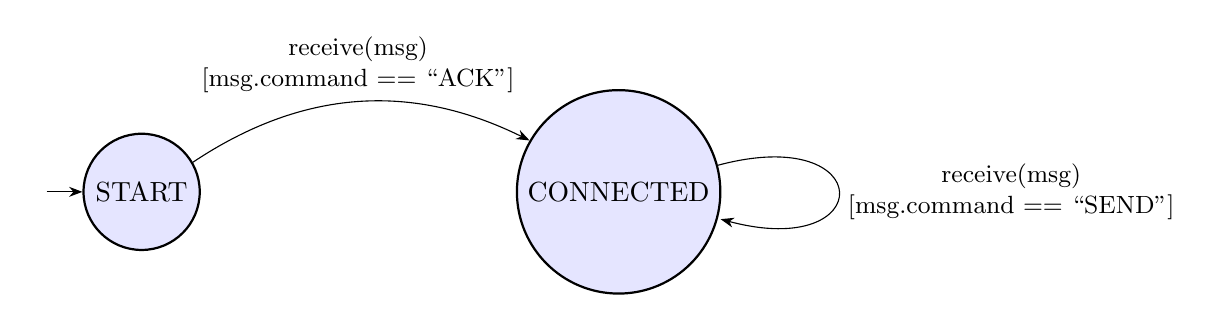
\begin{tikzpicture}[
  ->,>=Stealth,
  node distance=4cm,
  every state/.style={thick,fill=blue!10,minimum size=1.2cm},
  initial text={}
]
  \node[state,initial]  (S) {START};
  \node[state]          (C) [right=of S] {CONNECTED};

  \path (S) edge[bend left]
        node[above,font=\small,align=center]
          {receive(msg)\\$[$msg.command == ``ACK''$]$}
        (C)
        (C) edge[loop right]
        node[right,font=\small,align=center]
          {receive(msg)\\$[$msg.command == ``SEND''$]$}
        (C);
\end{tikzpicture}
\end{center}


% ═════════════════════════════════════════════════════════════════════════════
\section{Grammar Reference}
\label{sec:grammar}

This section provides the complete formal grammar of MaudeIR in
EBNF-like notation, closely mirroring the Lark parser specification.

\begin{lstlisting}[numbers=none,basicstyle=\ttfamily\footnotesize]
start       ::= statement*

statement   ::= import_stmt | config_stmt | type_decl
              | struct_decl | event_decl  | func_decl
              | machine_decl | test_decl

import_stmt ::= "import" STRING
config_stmt ::= "config" CNAME "." CNAME ":" type_expr
type_decl   ::= "type" CNAME ["=" type_expr]
struct_decl ::= "struct" CNAME "{" struct_field* "}"
struct_field::= CNAME ":" type_expr
event_decl  ::= "event" CNAME "(" [param_list] ")"
func_decl   ::= ["nondet"] "function" CNAME "(" [param_list] ")"
                "->" type_expr ["{" action_stmt* "}"]

type_expr   ::= CNAME ["[" type_expr ("," type_expr)* "]"]
param_list  ::= param ("," param)*
param       ::= CNAME ":" type_expr

machine_decl::= "machine" CNAME ["(" [param_list] ")"]
                "{" machine_member* "}"
machine_member
            ::= var_decl | state_decl | initial_decl
              | transition_decl | func_decl | event_decl

var_decl    ::= CNAME ":" type_expr ["=" expr]
state_decl  ::= "state" CNAME
initial_decl::= "initial" CNAME

transition_decl
            ::= "transition" CNAME "on" event_match
                ["[" guard "]"] "->" CNAME "{" action_stmt* "}"

event_match ::= CNAME "(" [event_args] ")"
event_args  ::= event_arg ("," event_arg)*
event_arg   ::= CNAME | STRING | CNAME ":" CNAME | struct_match

struct_match::= CNAME "{" [struct_match_fields] "}"
struct_match_fields
            ::= struct_match_field ("," struct_match_field)*
struct_match_field
            ::= CNAME ":" (CNAME | STRING | NUMBER
                          | struct_match | list_expr)

guard       ::= expr

action_stmt ::= assignment | return_stmt | expr_stmt
              | for_stmt | if_stmt
assignment  ::= assign_target "=" expr
assign_target
            ::= CNAME | CNAME "[" expr "]"
return_stmt ::= "return" expr
expr_stmt   ::= expr
for_stmt    ::= "for" CNAME "in" expr "{" action_stmt* "}"
if_stmt     ::= "if" expr "{" action_stmt* "}"

expr        ::= logic_or
logic_or    ::= logic_or "or" logic_and | logic_and
logic_and   ::= logic_and "and" comp_expr | comp_expr
comp_expr   ::= comp_expr COMP_OP math_expr | math_expr
math_expr   ::= math_expr MATH_OP term | term
term        ::= call_expr | index_expr | atom_expr
              | list_expr | "(" expr ")"

index_expr  ::= atom_expr "[" expr "]"
call_expr   ::= atom_expr "(" [expr_list] ")"
atom_expr   ::= CNAME ("." CNAME)* | STRING | NUMBER
              | "True" | "False"
list_expr   ::= "[" [expr_list] "]"
expr_list   ::= expr ("," expr)*

COMP_OP     ::= "==" | "!=" | "<" | ">" | "<=" | ">="
MATH_OP     ::= "+" | "-" | "*" | "/"

test_decl   ::= "test" STRING "{" test_stmt* "}"
test_stmt   ::= action_stmt | assert_stmt
assert_stmt ::= "assert" expr
\end{lstlisting}


% ═════════════════════════════════════════════════════════════════════════════
\appendix
\section{Quick Reference Card}
\label{app:quickref}

\begin{center}
\small
\begin{tabular}{@{}p{4cm}p{9cm}@{}}
\toprule
\textbf{Construct} & \textbf{Syntax} \\
\midrule
Import             & \texttt{import "file.model"} \\
Config parameter   & \texttt{config M.field: Type} \\
Type alias         & \texttt{type Name = Type} \\
Struct             & \texttt{struct Name \{ field: Type \}} \\
Event              & \texttt{event Name(p: Type)} \\
Function           & \texttt{function f(p: T) -> R \{ ... \}} \\
Nondet function    & \texttt{nondet function f(p: T) -> R} \\
Machine            & \texttt{machine M(p: T) \{ ... \}} \\
State              & \texttt{state S} \\
Initial state      & \texttt{initial S} \\
Variable           & \texttt{name: Type = expr} \\
Transition         & \texttt{transition S1 on evt(...) [guard] -> S2 \{ ... \}} \\
Test               & \texttt{test "name" \{ ... \}} \\
Assertion          & \texttt{assert expr} \\
Conditional        & \texttt{if expr \{ ... \}} \\
Loop               & \texttt{for v in expr \{ ... \}} \\
Log                & \texttt{log(LEVEL, "msg \{var\}")} \\
Delete             & \texttt{del(collection, key)} \\
Length             & \texttt{len(collection)} \\
\bottomrule
\end{tabular}
\end{center}

% ═════════════════════════════════════════════════════════════════════════════
\section{Maude Output Module Structure}
\label{app:maude-modules}

\begin{center}
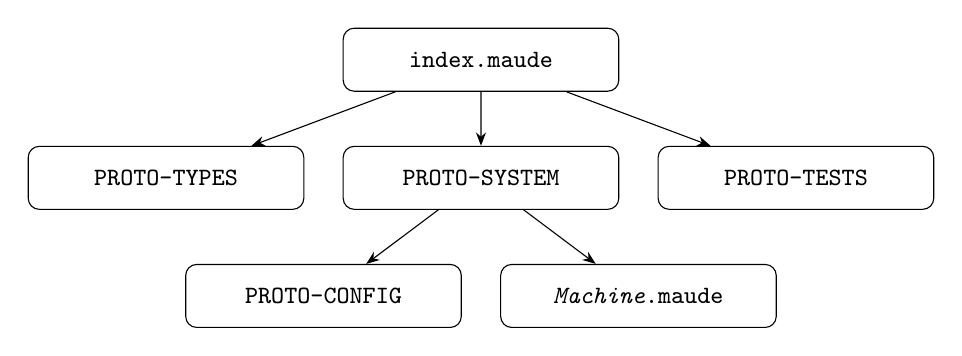
\begin{tikzpicture}[
  every node/.style={draw, rounded corners, minimum width=3.5cm,
                     minimum height=0.8cm, font=\small\ttfamily},
  level 1/.style={sibling distance=4cm},
  edge from parent/.style={draw,->,>=Stealth},
  grow=down, level distance=1.5cm
]
  \node {index.maude}
    child { node {PROTO-TYPES} }
    child { node {PROTO-SYSTEM}
      child { node {PROTO-CONFIG} }
      child { node {\textit{Machine}.maude} }
    }
    child { node {PROTO-TESTS} };
\end{tikzpicture}
\end{center}

\begin{itemize}[leftmargin=1.5em]
  \item \textbf{PROTO-TYPES} (\texttt{fmod}): Struct sorts, constructors,
        and field projection equations.
  \item \textbf{PROTO-SYSTEM} (\texttt{omod}): Message operators, logging
        infrastructure, map operations, and function mocks.
  \item \textbf{PROTO-CONFIG} (\texttt{fmod}): Named constants populated
        from the YAML configuration.
  \item \textbf{\textit{Machine}} (\texttt{omod}): Class declaration,
        state sort, and rewrite rules per machine.
  \item \textbf{PROTO-TESTS} (\texttt{omod}): Test configurations with
        \texttt{search} commands.
\end{itemize}

\end{document}
